\subsection*{Exercice 1 : modèles digitaux}

\begin{figure}[!htbp]
   \centering
   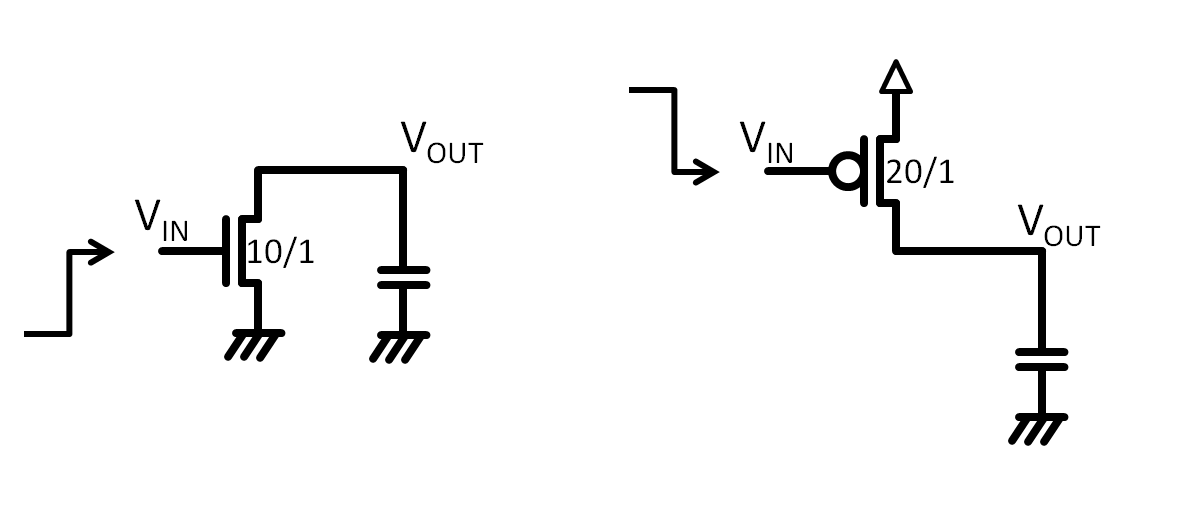
\includegraphics[width=10cm]{figure/fig7-1.png}
   \caption{Exercice 1}
   \label{fig7-1}
\end{figure}

Calculez les délais à 50\% des transitions symbolisées sur la figure~\ref{fig7-1}
pour des transistors à canaux court en technologie 50nm avec \cox=62.5aF/$\mu m^2$,
$R_n$=34k$\Omega\mu$m et $R_p$=68k$\Omega\mu$m.
Les tailles des NMOS valent $W=10\mu$m et $L=1\mu$m tandis que celles des PMOS valent
$W=20\mu$m et $L=1\mu$m.

\subsection*{Exercice 2 : inverseur CMOS}

On considère une chaîne d'inverseurs CMOS identiques avec ses pistes d'interconnexion
en technologie 0.18$\mu$m, comme représenté à la figure~\ref{fig7-2}. Voici les paramètres
technologiques :

\begin{center}
$
	\begin{array}{l l l}
		L_{min} = 0.18 \mu m 	& V_{DD} = 1.8 V 		& V_{t0,n} = |V_{t0,p} | = 0.5 V \\
		\mu_n = 0.04 m^2/Vs 	& \mu_p = 0.02 m^2/Vs	& C_{ox} = 5 fF/\mu m^2 \\
		C_{rout} = 10fF			&						& \\
	\end{array}
$
\end{center}

\begin{figure}[!htbp]
   \centering
   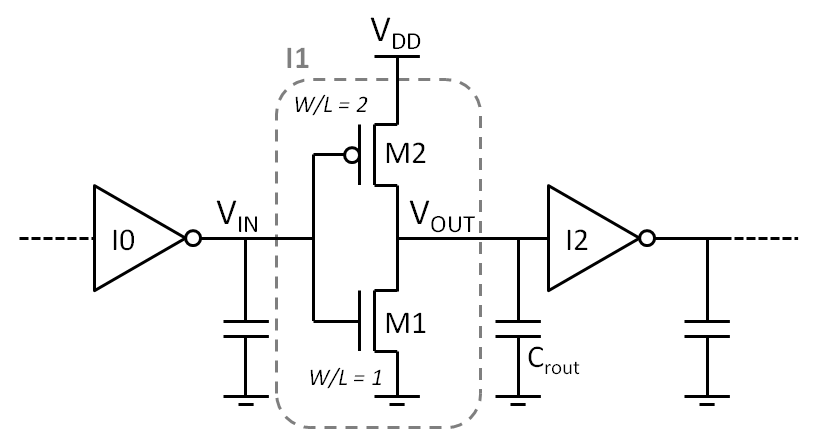
\includegraphics[width=10cm]{figure/fig7-2.png}
   \caption{Exercice 1}
   \label{fig7-2}
\end{figure}

\emph{Analyse DC}
\begin{enumerate}
	\item Pour une transition infiniment lente à l'entrée de I1, déterminez le régime de
	fonctionnement de M1 et M2 ainsi que la tension \vout en fonction de \vin.
\end{enumerate}

\emph{Délai de propagation}
\begin{enumerate}
	\setcounter{enumi}{1}
	\item Comme estimation du délai de propagation ($t_p$) de I1, on vous demande de
	calculer le temps de descente de \vout à 50\% lors d'un flanc montant sur \vin
	($t_{PHL}$). Pour ce faire, remplacer M1 et M2 par des éléments plus simples
	(résistance, sources) en fonction du régime de fonctionnement. On suppose que
	le flanc sur \vin est idéal et on néglige les capacités parasites.
	\item On souhaite simplifier le calcul du délai de propagation en remplaçant M1
	par une résistance équivalente $R_{eq}$ qui donne la même valeur de délai que
	celle trouvée précédemment. Pour ce faire, on vous demande de trouver un facteur
	de fitting k pour exprimer $R_{eq}$ en fonction de la résistance en mode linéaire
	:\\ $R_{eq}$ = k $R_{lin}$ .
\end{enumerate}

\emph{Scaling de la technologie CMOS}
\begin{enumerate}
	\setcounter{enumi}{3}
	\item On considère cette fois une technologie 65nm avec les paramètres ci-dessous.
	Calculer le délai sur base de la formule obtenue au point c). Négliger les capacités parasites.

	\begin{center}
	$
		\begin{array}{l l l}
			L_{min} = 65 nm 		& V_{DD} = 1.2V 		&V_{t0,n} = |V_{t0,p}| = 0.4V \\
			\mu_n = 0.05 m^2/Vs 	& \mu_p= 0.025 m^2/Vs	& C_{ox} = 7 fF/\mu m^2 \\
			C_{rout} = 2fF			&						& \\
		\end{array}
	$
	\end{center}
\end{enumerate}

\subsection*{Exercice 3 : Logique de passage}
On considère les 3 implémentations d'un multiplexeur 2 vers 1 de la figure~\ref{fig7-3} :
transmission gate, pass gate et static CMOS gate. La fonction logique associée est :
Y = (Sel.A) + ($\overline{Sel}$.B) et la technologie considérée est une technologie
0.18 $\mu$m avec les paramètres suivants:

\begin{center}
$
	\begin{array}{l l l}
		L_{min} = 0.18 \mu m 	& V_{DD} = 1.8 V 		& V_{t0,n} = |V_{t0,p} | = 0.5 V \\
		\mu_n = 0.04 m^2/Vs 	& \mu_p = 0.02 m^2/Vs	& C_{ox} = 5 fF/\mu m^2 \\
		C_{rout} = 10fF			&						& \\
	\end{array}
$
\end{center}

\begin{figure}[!htbp]
   \centering
   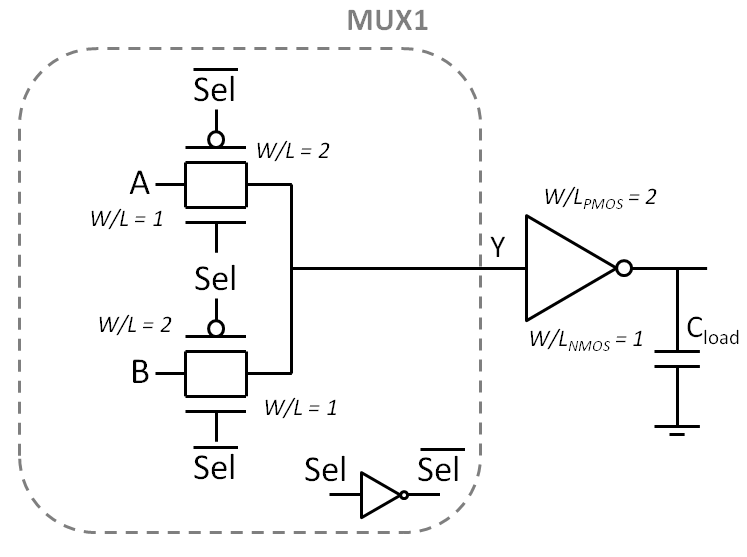
\includegraphics[width=9cm]{figure/fig7-3-1.png}
	 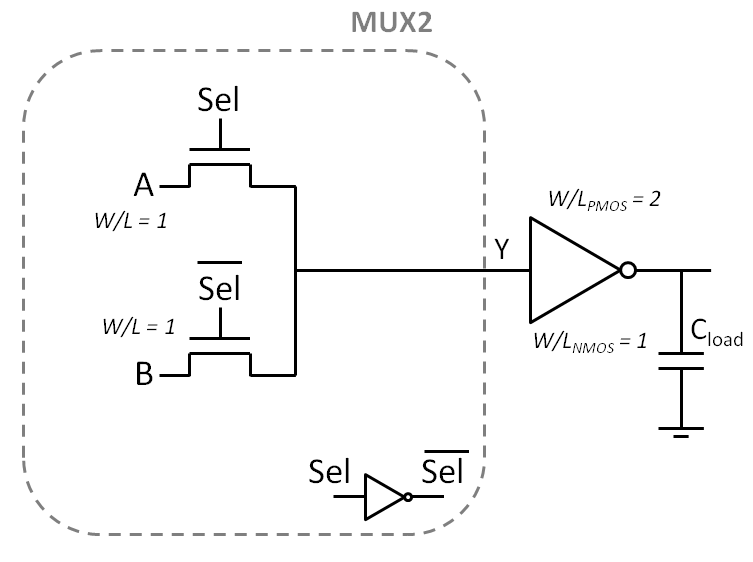
\includegraphics[width=9cm]{figure/fig7-3-2.png}
	 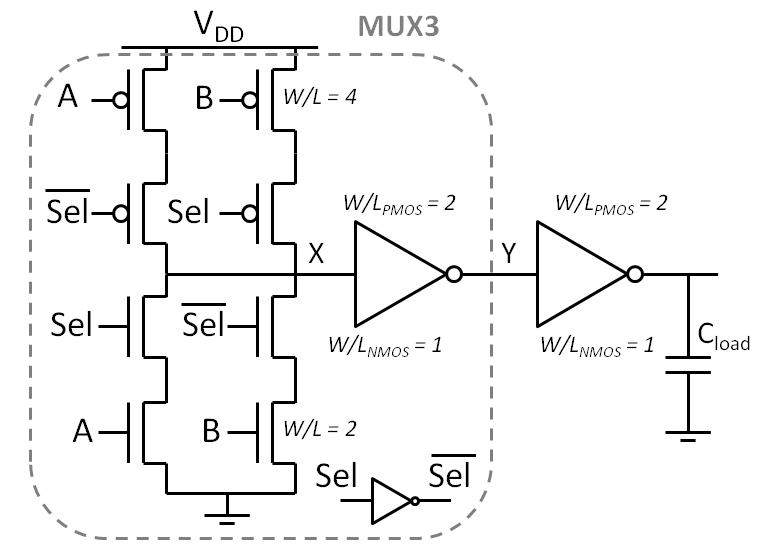
\includegraphics[width=9cm]{figure/fig7-3-3.png}
   \caption{Exercice 1}
   \label{fig7-3}
\end{figure}

\begin{enumerate}
	\item Déterminer les tensions des niveaux logiques haut ($V_{OH}$) et bas ($V_{OL}$) de
	la sortie Y pour chacun de ces multiplexeurs.
	\item Calculez le temps de décharge à 50\% ($t_{PHL}$) de la capacité $C_{load}$ par
	l'inverseur de l'étage suivant, suite à un flanc montant à la sortie Y. Considérez une
	résistance équivalente pour les transistors passant du régime saturé au linéaire de
	$R_{eq}$ = 2.5 $R_{lin}$ et négliger toutes les capacités parasites.
\end{enumerate}